\documentclass[UTF8,zihao=-4]{ctexart}
\usepackage[a4paper,margin=2.5cm]{geometry}
\usepackage{amsmath, amssymb, amsthm}
\usepackage{bm}
\usepackage{hyperref}
\usepackage{graphicx}
\usepackage{caption}
\usepackage{listings}
\usepackage{xcolor}
\usepackage{float}
\usepackage{booktabs}
\usepackage{longtable}
\usepackage{multirow}
\usepackage{placeins}
\graphicspath{{figures/}}

% 代码样式
\lstdefinestyle{code}{
  basicstyle=\ttfamily\small,
  numbers=left,
  numberstyle=\tiny,
  numbersep=8pt,
  keywordstyle=\color{blue},
  commentstyle=\color{teal!70!black},
  stringstyle=\color{orange!70!black},
  showstringspaces=false,
  breaklines=true,
  frame=single,
  framerule=0.3pt,
  rulecolor=\color{black!15}
}
\lstset{style=code}

\title{训练框架与体系化流程:Transformers、分布式引擎与监控实践}
\author{}
\date{\today}

\begin{document}
\maketitle

\section{Hugging Face Transformers 全流程}
\subsection{工作流概览}
Hugging Face Transformers 生态提供了从数据准备、模型配置到评估与部署的完整闭环。图\ref{fig:hf_pipeline_cn} 总结了标准流程:从数据集加载到模型发布,各环节均可插拔扩展。
\begin{figure}[H]
  \centering
  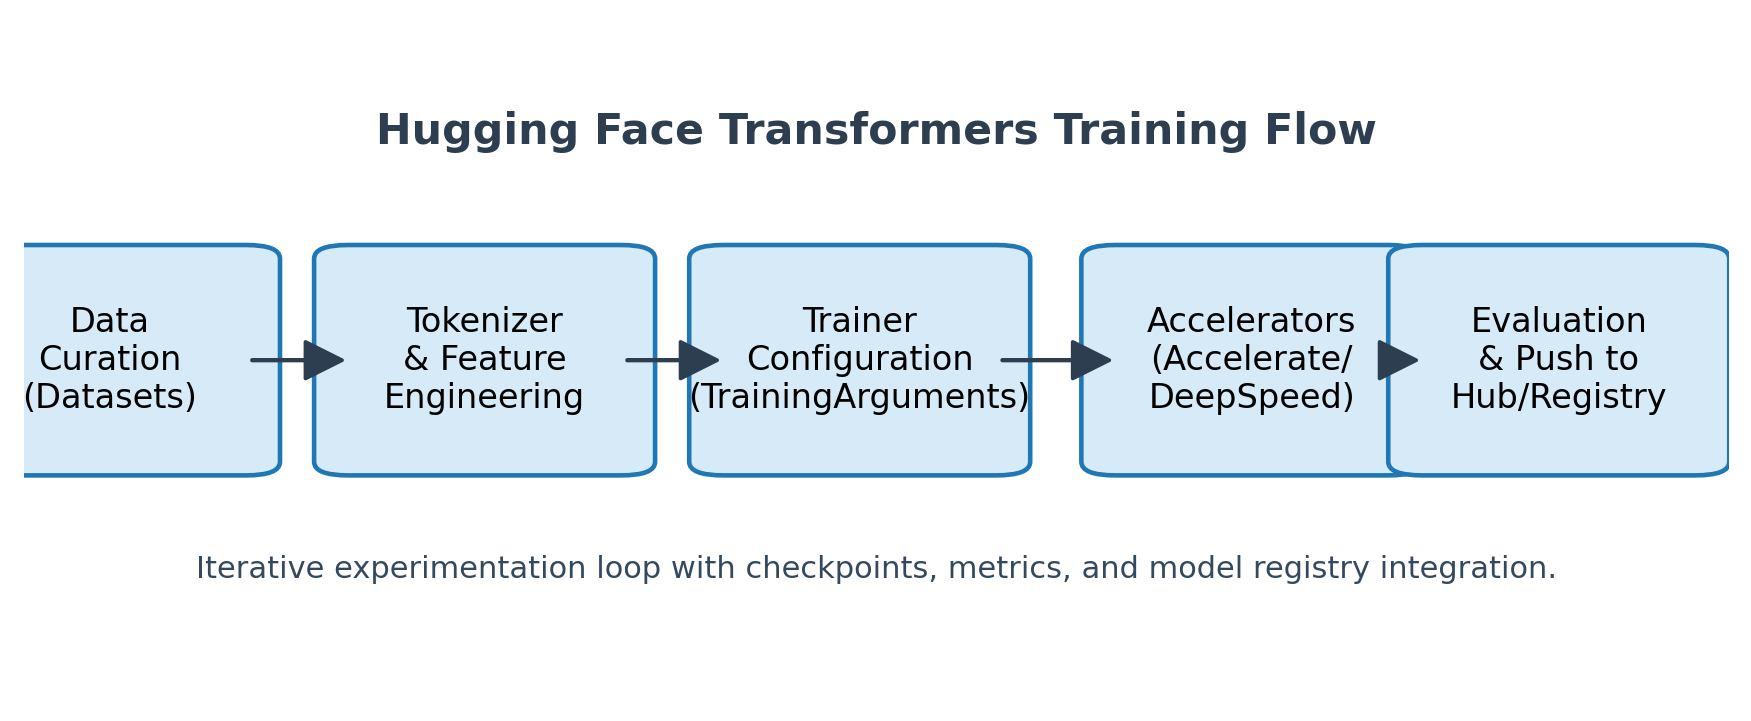
\includegraphics[width=0.9\textwidth]{hf_training_pipeline.png}
  \caption{Hugging Face Transformers 训练流程:数据、特征工程、训练配置、加速器集成与模型发布。}
  \label{fig:hf_pipeline_cn}
\end{figure}
核心步骤:
\begin{enumerate}
  \item \textbf{数据集与特征工程:} 使用 \texttt{datasets} 库加载文件或远程数据集,支持流式读取、分片加载和 `map`、`filter`、`train\_test\_split` 等操作。配合 Tokenizer 完成分词、截断与动态填充,确保批次内形状一致。
  \item \textbf{模型与配置:} 通过 \texttt{AutoModelForCausalLM}、\texttt{AutoModelForSeq2SeqLM} 等自动选择模型结构,使用 \texttt{AutoConfig} 调整隐藏层、注意力头、KV 缓存等参数。
  \item \textbf{训练器(Trainer):} \texttt{Trainer} 与 \texttt{TrainingArguments} 提供梯度累积、学习率调度、混合精度(fp16/bf16)、日志记录、多 GPU/TPU 支持。可通过 Callback 注入自定义逻辑(如模型保存策略、早停、指标上报)。
  \item \textbf{评估与部署:} 使用 \texttt{Trainer.evaluate}、\texttt{Trainer.predict} 进行指标计算,集成 \texttt{datasets.load\_metric} 或 \texttt{evaluate} 库。训练完成后可将模型权重、Tokenizer、配置打包并推送至 Hugging Face Hub 或内部模型仓库。
\end{enumerate}

\subsection{高效训练技巧}
\begin{itemize}
  \item \textbf{数据流优化:} 利用 streaming dataset + `DataCollator` 降低内存占用;在 TPU 场景使用 `IterableDataset` 与 `Shard` 保证数据分布均匀。
  \item \textbf{混合精度与编译:} `bf16` 对 A100、H100 等 GPU 数值稳定性更佳;配合 `torch.compile`、`FlashAttention`、`DeepSpeed` 集成提升性能。
  \item \textbf{参数高效微调:} 通过 `peft` 库集成 LoRA、QLoRA、Adapter 等技术,减少显存需求并加快迭代速度。
  \item \textbf{自动化实验:} 借助 \texttt{HfArgumentParser} 配置 YAML/JSON 文件,实现可重复实验;结合 `wandb`、`mlflow` 记录超参、日志与模型检查点。
\end{itemize}

\subsection{典型代码模版}
\begin{lstlisting}[language=Python,caption={使用 Trainer 进行指令微调示例}]
from datasets import load_dataset
from transformers import AutoTokenizer, AutoModelForCausalLM, TrainingArguments, Trainer
from transformers import DataCollatorForLanguageModeling

model_name = "Qwen/Qwen2-7B-Instruct"
tokenizer = AutoTokenizer.from_pretrained(model_name, use_fast=True)
dataset = load_dataset("json", data_files={"train": "train.jsonl", "eval": "eval.jsonl"})

def preprocess(example):
    return tokenizer(example["prompt"], text_target=example["response"], truncation=True)

tokenized = dataset.map(preprocess, batched=True, remove_columns=dataset["train"].column_names)

collator = DataCollatorForLanguageModeling(tokenizer, mlm=False)
model = AutoModelForCausalLM.from_pretrained(model_name, torch_dtype="bfloat16")

args = TrainingArguments(
    output_dir="outputs/qwen-sft",
    per_device_train_batch_size=4,
    gradient_accumulation_steps=8,
    num_train_epochs=3,
    learning_rate=2e-5,
    logging_steps=10,
    evaluation_strategy="steps",
    eval_steps=200,
    save_steps=200,
    report_to=["wandb"],
    bf16=True,
    push_to_hub=True,
)

trainer = Trainer(
    model=model,
    args=args,
    train_dataset=tokenized["train"],
    eval_dataset=tokenized["eval"],
    data_collator=collator,
)

trainer.train()
\end{lstlisting}

\section{DeepSpeed / Megatron-LM / ColossalAI}
\subsection{架构能力对比}
DeepSpeed、Megatron-LM、ColossalAI 聚焦在超大规模模型训练的并行策略与内存优化。图\ref{fig:distributed_landscape_cn} 对比了三者的核心能力:
\begin{figure}[H]
  \centering
  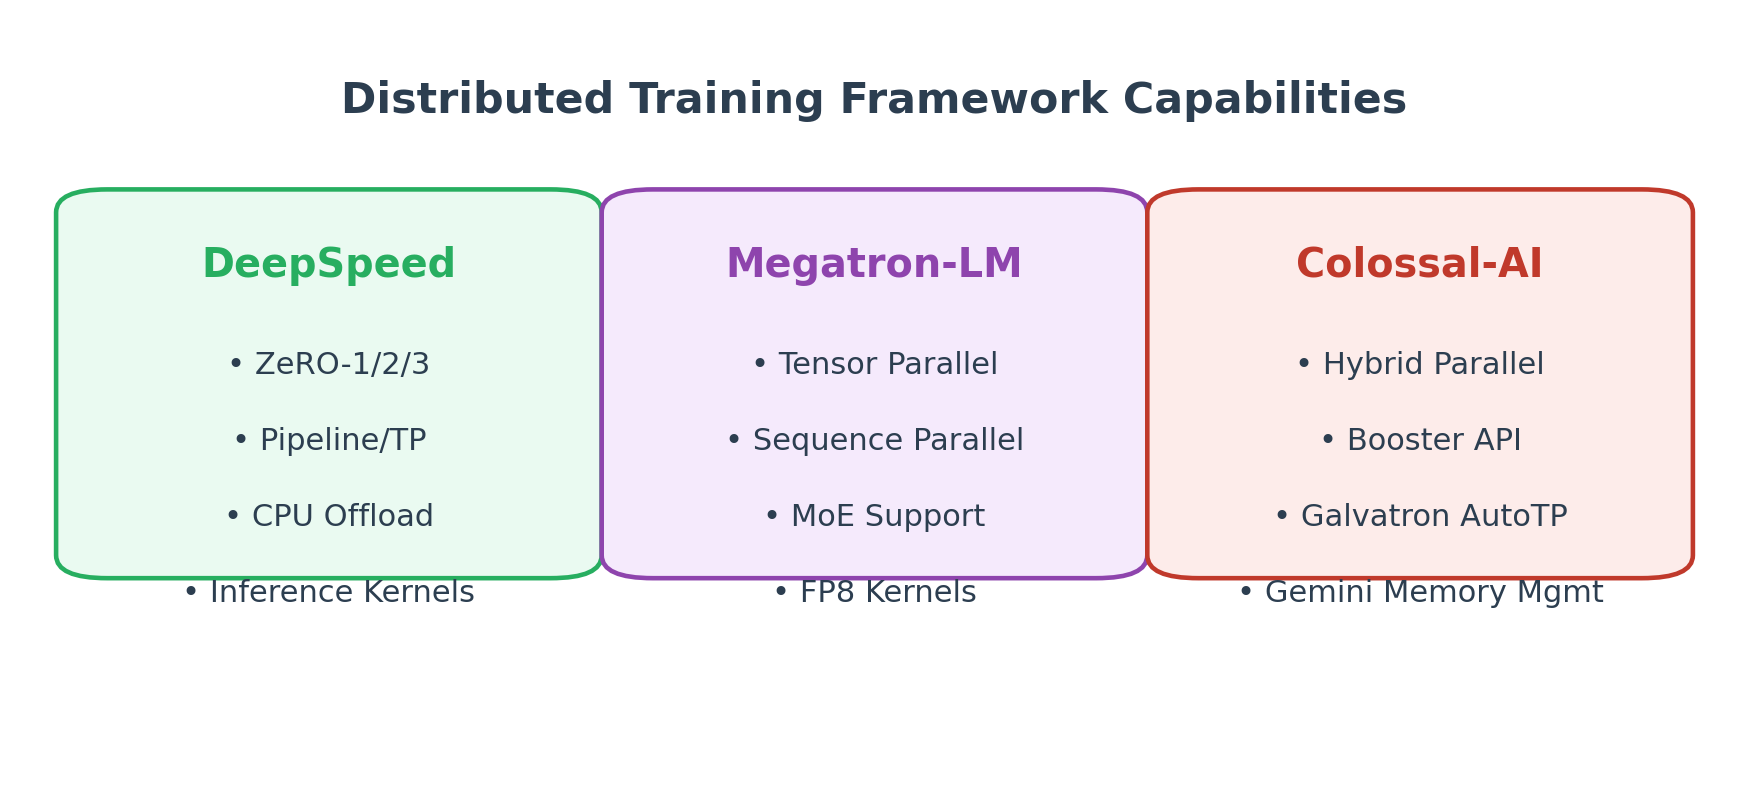
\includegraphics[width=0.9\textwidth]{distributed_frameworks.png}
  \caption{主流分布式训练框架能力对比。}
  \label{fig:distributed_landscape_cn}
\end{figure}
\begin{longtable}{p{3cm}p{5cm}p{6cm}}
\toprule
框架 & 核心特性 & 适用场景 \\
\midrule
DeepSpeed & ZeRO-1/2/3、ZeRO-Offload、量化感知训练、Inference Engine & 大规模自回归模型训练与推理;需要多节点内存分片 \\
Megatron-LM & Tensor 并行、Sequence 并行、Pipeline 并行、MoE 支持 & GPT/MoE 超大模型预训练;高性能 GPU 集群 \\
ColossalAI & Hybrid Parallel、Gemini 动态内存管理、Booster API、自动张量并行(Galvatron) & 工程灵活性高的科研与企业场景;需要自动搜索并行策略 \\
\bottomrule
\end{longtable}

\subsection{ZeRO 与混合并行}
ZeRO (Zero Redundancy Optimizer)通过拆分优化器状态、梯度、参数实现线性扩展:
\begin{itemize}
  \item \textbf{ZeRO-1:} 优化器状态(如 Adam 的动量)切分到不同 GPU。
  \item \textbf{ZeRO-2:} 梯度也切分,减少通信与显存占用。
  \item \textbf{ZeRO-3:} 参数切分,训练时按需广播,从而支持 100B+ 模型。
\end{itemize}
与 Pipeline Parallel、Tensor Parallel 结合构成混合并行(Hybrid Parallel),同时利用数据并行、流水线并行与张量并行各自优势。

\subsection{实践策略}
\begin{itemize}
  \item \textbf{推进顺序:} 先确定 ZeRO 阶段,再根据模型结构选择张量并行维度(如注意力头数可整除张量并行度),最后决定流水线切分层数。
  \item \textbf{通信优化:} 使用 NCCL + SHARP + NVLink/NVSwitch;在多机环境启用异步梯度压缩或 1-bit Adam。
  \item \textbf{容错:} DeepSpeed Checkpoint Engine 支持阶段性恢复;Megatron-LM 提供张量并行容错;ColossalAI 可通过 Gemini 快照恢复模型状态。
  \item \textbf{MoE:} Megatron-Core 与 DeepSpeed MoE 支持专家并行(EP),需结合 Top-$k$ gating、容量因子、路由正则等参数调优 load balance。
\end{itemize}

\section{Checkpoint 合并、转换与裁剪}
\subsection{常见需求}
随着模型规模与微调任务增多,需要灵活处理不同来源的 checkpoint:
\begin{itemize}
  \item \textbf{合并 LoRA 权重:} 将 LoRA 适配器融入基础模型,方便推理部署;
  \item \textbf{多分片权重合并:} 分布式训练时的张量并行权重需要恢复为单份以便部署;
  \item \textbf{格式转换:} 例如从 PyTorch `.bin/.safetensors` 转换为 `.gguf`、TensorRT-LLM engine、ONNX 等;
  \item \textbf{权重裁剪:} 截断最大上下文、移除冗余位置编码、删除未使用的适配器。
\end{itemize}

\subsection{工具与流程}
\begin{longtable}{p{3cm}p{4cm}p{6cm}}
\toprule
工具 & 功能 & 注意事项 \\
\midrule
\texttt{merge\_lora.py} (peft) & 将 LoRA 合并进基础模型 & 合并后需保存为 \texttt{safetensors},防止精度丢失 \\
\texttt{transformers.convert} & 各模型格式互转(Bloom、OPT、GPT-NeoX) & 需指定目标权重分片大小和词表路径 \\
\texttt{ggml/llama.cpp} 转换脚本 & 转换为 gguf/ggml 量化格式 & 先执行量化,再验证困惑度变化 \\
TensorRT-LLM \texttt{trtllm-build} & 编译 FP16/INT8 engine & 准备校准数据、配置 KV Cache 策略 \\
\bottomrule
\end{longtable}

\subsection{案例:合并 LoRA 并导出 ONNX}
\begin{lstlisting}[language=Python,caption={合并 LoRA 并导出 ONNX 推理图}]
from transformers import AutoModelForCausalLM, AutoTokenizer
from peft import PeftModel
import torch

base_model = "meta-llama/Llama-3-8b"
lora_path = "outputs/llama-sft-lora"
export_path = "artifacts/llama3-sft"

tokenizer = AutoTokenizer.from_pretrained(base_model)
model = AutoModelForCausalLM.from_pretrained(base_model, torch_dtype=torch.float16)
model = PeftModel.from_pretrained(model, lora_path)
model = model.merge_and_unload()  # 合并 LoRA 权重
model.save_pretrained(export_path, safe_serialization=True)
tokenizer.save_pretrained(export_path)

dummy = torch.randint(0, tokenizer.vocab_size, (1, 256), dtype=torch.long)
torch.onnx.export(
    model,
    (dummy,),
    f"{export_path}/model.onnx",
    input_names=["input_ids"],
    output_names=["logits"],
    dynamic_axes={"input_ids": {0: "batch", 1: "seq"}},
    opset_version=18,
)
\end{lstlisting}
导出后需借助 \texttt{onnxruntime} 或 TensorRT 验证功能正确性,并对 logits 进行精度对比。

\section{分布式训练与监控工具(W\&B, TensorBoard)}
\subsection{监控指标设计}
在大规模训练中,监控不仅涵盖损失曲线,还应关注:
\begin{itemize}
  \item \textbf{系统指标:} GPU/CPU 利用率、显存占用、网络带宽、I/O 吞吐;
  \item \textbf{训练指标:} Loss、Perplexity、梯度范数、学习率、梯度裁剪比例;
  \item \textbf{分布式通信:} AllReduce 时间、ZeRO 同步时延、参数更新延迟;
  \item \textbf{质量评估:} Eval 指标、BLEU/BERTScore、人类偏好打分、自动对齐指标。
\end{itemize}

\subsection{Weights \& Biases 集成}
W\&B 通过 \texttt{wandb.init} 和 \texttt{wandb.log} 与 \texttt{Trainer}、DeepSpeed、Accelerate 无缝集成。常见实践:
\begin{itemize}
  \item 使用 \texttt{wandb.Table} 存储样例输出、评估日志;
  \item 通过 Artifact 管理模型权重与数据版本;
  \item 设置 Sweeps 运行超参搜索,与 Ray Tune、Optuna 结合;
  \item 在多机场景启用 `WANDB_START_METHOD=thread` 防止进程冲突。
\end{itemize}

\subsection{TensorBoard 与自定义可视化}
TensorBoard 提供简单可靠的跨框架可视化:
\begin{itemize}
  \item \textbf{SummaryWriter:} 在 PyTorch 中通过 `add_scalar`、`add_histogram`、`add_graph` 记录各类信息;
  \item \textbf{分布式兼容:} 只在 rank 0 进程写日志,或使用 `gloo`/`file` 后端聚合;
  \item \textbf{Embedding 可视化:} 记录词向量或分类器隐表示的降维结果,分析模型学习效果;
  \item \textbf{Profile 插件:} 跟踪 GPU Kernel 时间、内存拷贝、通信开销。
\end{itemize}

\subsection{告警与自动化}
监控不仅用于观察,还需触发告警与自动化响应:
\begin{itemize}
  \item 结合 Prometheus + Alertmanager,对显存溢出、梯度爆炸、loss Nan 设置阈值;
  \item 将训练指标同步至 Grafana 看板,与集群调度系统(如 Kubernetes)共享告警;
  \item 使用 `wandb.alert` 或 Slack/Webhook 通知异常;
  \item 在训练脚本中根据监控信号实现自动降级(调整批大小、切换 ZeRO 阶段)或安全停止。
\end{itemize}

\section*{实践建议}
\begin{itemize}
  \item 在项目初期建立统一的配置格式和脚本模板,确保数据处理、训练、评估、导出流程可复现。
  \item 为每个分布式框架准备最小可运行示例,验证通信、ZeRO、并行策略后再扩展到完整规模。
  \item Checkpoint 操作要搭配校验流程:计算哈希、对比困惑度、执行黑盒推理测试,避免部署不一致。
  \item 将监控数据与实验元数据(超参、Git commit、数据版本)绑定,方便后续追踪与审计。
\end{itemize}

\section*{参考文献}
\begin{itemize}
  \item Rajbhandari et al. ``ZeRO: Memory Optimizations Toward Training Trillion Parameter Models.'' SC, 2020.
  \item Narayanan et al. ``Efficient Large-Scale Language Model Training on GPU Clusters Using Megatron-LM.'' NeurIPS, 2021.
  \item Jiang et al. ``Colossal-AI: A Unified Deep Learning System For Large-Scale Parallel Training.'' arXiv, 2022.
  \item Hugging Face. ``Transformers Documentation.'' 2024.
  \item Biewald. ``Experiment Tracking with Weights and Biases.'' ODSC, 2020.
\end{itemize}

\end{document}

